\documentclass[12pt, letterpaper, parskip = full]{article}
\usepackage[mmddyyyy]{datetime}

\usepackage[utf8]{inputenc}
\usepackage{amsmath}
\usepackage{mathpazo}
\usepackage{eulervm}

\usepackage[margin=1in]{geometry}
\linespread{1.20}
\usepackage{enumerate}
\usepackage{enumitem}
\usepackage{listings}
\usepackage[T1]{fontenc}
\usepackage{amsfonts}
\usepackage{amssymb}
\usepackage{amsthm}
\usepackage{multirow,array}
\usepackage{graphicx}
\usepackage{physics}
\usepackage{bm}
\usepackage{tikz}
\usepackage{breqn}
\usepackage[longnamesfirst]{natbib}
\usepackage{comment}
\usepackage{setspace}
\usepackage{hyperref}

\graphicspath{{Images/}}

\newtheorem{theorem}{Theorem}
\newtheorem{corollary}{Corollary}
\newtheorem{lemma}{Lemma}
\newtheorem{definition}{Definition}
\newtheorem{axiom}{Axiom}
\newcommand{\e}{\mathrm{e}}
\newcommand{\Var}{\mathrm{Var}}
\newcommand{\Ex}[1]{\mathbb{E}\left[#1\right]}
\renewcommand{\Pr}[1]{\mathbb{P}(#1)}
\newcommand{\plim}{\mathrm{plim}}
\newcommand{\pc}[1]{\frac{\dot{#1}(t)}{#1(t)}}
\renewcommand\qedsymbol{$\blacksquare$}

\title{Homework 5}
\author{Alejandro Flores-Brown}

\begin{document}

  \maketitle

  \section{Problem 1}

  The given income process is negative for some ages, so we cannot simply take logs to transform income. Therefore I set income to be \(-4\) when estimated income is negative. Otherwise, the code is as normal. The policy function is given below.

  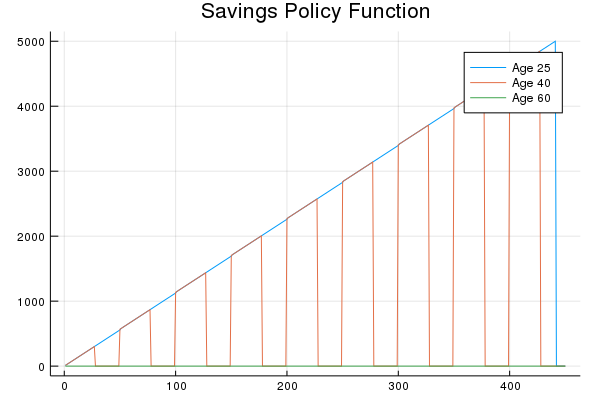
\includegraphics[scale=0.5]{f1.png}

  \subsection{Part B}

  I now simulate the lifetime consumption, saving, and income for one individual.

  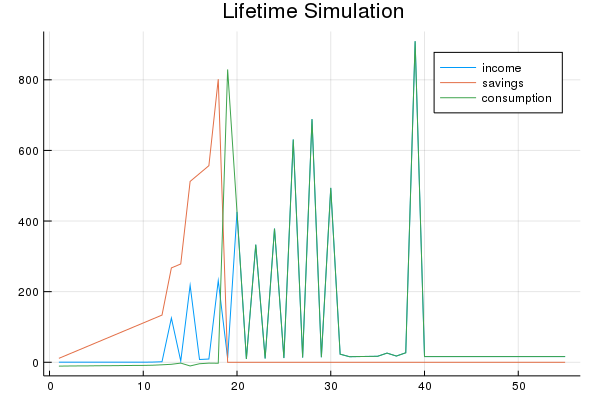
\includegraphics[scale=0.25]{f2.png}

  \subsection{Part C}

  I next simulate the lifetime consumption, saving, and income for 10000 individuals.

  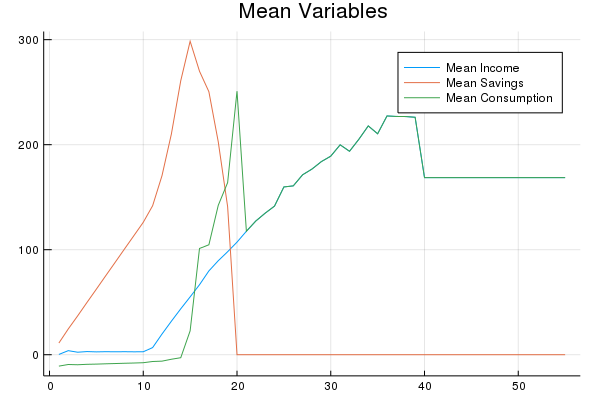
\includegraphics[scale=0.5]{f3.png}

  Variances are given below.

  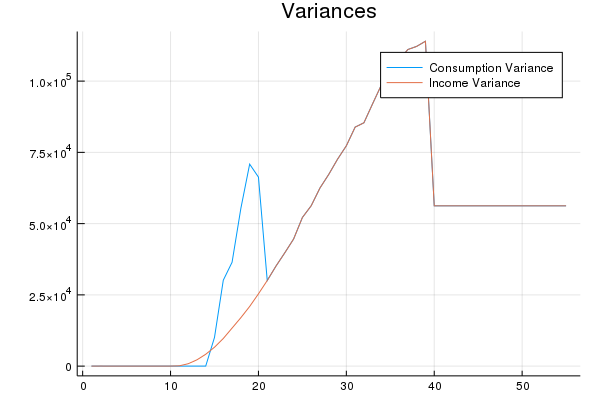
\includegraphics[scale=0.5]{f5.png}

  \subsection{Part D}

  I next do the same simulation with a lower borrowing constraint.

  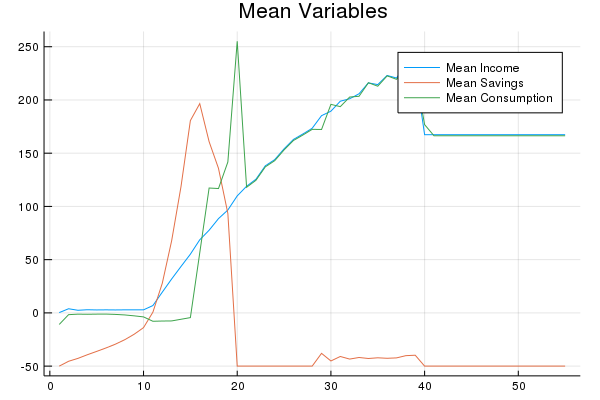
\includegraphics[scale=0.5]{f4.png}

  Variances are given below.

  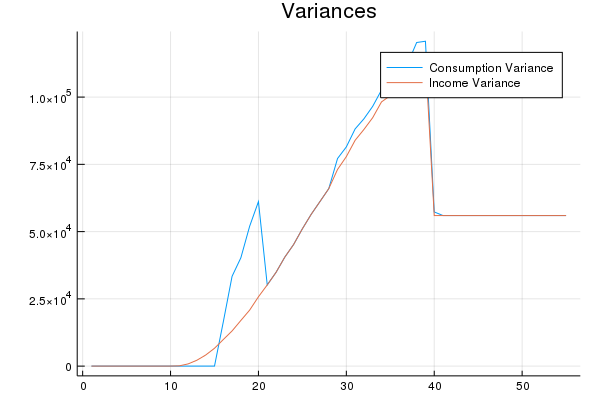
\includegraphics[scale=0.5]{f6.png}

  \newpage

  \appendix

  Julia Code

  \begin{lstlisting}[breaklines]

  using Plots, LinearAlgebra

  n_l=25
  n_h=80
  mn = n_h - n_l

  n_t=65
  sigma=2
  Gamma=0.92
  r=0.02
  R=1+r
  z=[log(15); log(80); log(500)]
  Gamma=[0.6 0.35 0.05;0.1 0.8 0.1;0.05 0.35 0.6]

  f = zeros(mn)
  for i=1:mn
      if -1.0135+0.1086*i-0.001122*i^2 > 0
          f[i] = log(-1.0135+0.1086*i-0.001122*i^2)
      else
          f[i] = -4
      end
  end

  epsilon = [log(0.8) log(1.2)]
  pepsilon = [0.5 0.5]
  exepsilon = dot(pepsilon,epsilon)
  m1 = length(epsilon)

  Piz = [1/3 1/3 1/3] * Gamma^1000
  exz = dot(Piz,z)
  m2 = length(z)

  a_l = 0
  a_h = 5000
  m3 = 450

  function calval(age::Int,income::Int,shock::Int,assets::Int,valfun::Array{Float64,4},a::Array{Float64,1})
      local Rz = 0
      local v = 0
      local s = 0

      if age+25>64
          Rz = 0.7*exp(z[income] + f[n_t - 25])
          s=1
      end

      if age+25==80
          if R*a[assets] +Rz < 0
              v= (1/(1-sigma))*(R*a[assets]+Rz)^(1-sigma)
          else
              v = -999999-99*abs(R*a[assets]+Rz)
          end
      elseif age+25>65
          local V1 = zeros(m3)
          for i=1:m3
              if R*a[assets] + Rz - a[i]<0
                  V1[i] = -999999-99*abs(R*a[assets]+Rz-a[i])
              else
                  V1[i]=(1/(1-sigma))*(R*a[assets]+Rz-a[i])^(1-sigma)+Gamma*valfun[i,income,shock,age-1]
              end
          end
          helpv = findmax(V1)
          v = helpv[1]
          s = helpv[2]
      elseif age+25 == 65
          local V1 = zeros(m3)
          for i=1:m3
              if R*a[assets]+exp(z[income]+f[n_t-25]+epsilon[shock])-a[i]<0
                  V1[i] = -999999-99*abs(R*a[assets]+exp(z[income]+f[age]+epsilon[shock])-a[i])
              else
                  V1[i]=(1/(1-sigma))*(R*a[assets]+exp(z[income]+f[age]+epsilon[shock])-a[i])^(1-sigma)+Gamma*valfun[i,income,shock,age-1]
              end
          end
          v = maximum(V1)
      elseif age+25 > 25
          local V1 = zeros(m3)
          for i=1:m3
              if R*a[assets]+exp(z[income]+f[n_t-age-25]+epsilon[shock])-a[i]<0
                  V1[i] = -999999-99*abs(R*a[assets]+exp(z[income]+f[age]+epsilon[shock])-a[i])
              else
                  local n = n_t - age - 24
                  V1[i]=(1/(1-sigma))*(R*a[assets]+exp(z[income]+f[age]+epsilon[shock])-a[i])^(1-sigma)
                  +Gamma*(Gamma[income,1]*(0.5*valfun[i,1,1,n] + 0.5*valfun[i,1,2,n]) + Gamma[income,2]*(0.5*valfun[i,2,1,n]+0.5*valfun[i,2,2,n])
                  + Gamma[income,3]*(0.5*valfun[i,3,1,n]+0.5*valfun[i,3,2,n]) )
              end
          end
          helpv = findmax(V1)
          v = helpv[1]
          s = helpv[2]
      else
          local V1 = zeros(m3)
          for i=1:m3
              if exp(z[income]+f[n_t-age-25]+epsilon[shock])-a[i]<0
                  V1[i] = -999999-99*abs(exp(z[income]+f[age]+epsilon[shock])-a[i])
              else
                  local n = n_ret - age - 24
                  V1[i]=(1/(1-sigma))*(exp(z[income]+f[age]+epsilon[shock])-a[i])^(1-sigma)
                  +Gamma*(Gamma[income,1]*(0.5*valfun[i,1,1,n] + 0.5*valfun[i,1,2,n]) + Gamma[income,2]*(0.5*valfun[i,2,1,n]+0.5*valfun[i,2,2,n])
                  + Gamma[income,3]*(0.5*valfun[i,3,1,n]+0.5*valfun[i,3,2,n]) )
              end
          end
          helpv = findmax(V1)
          v = helpv[1]
          s = helpv[2]
      end
      return v,s
  end

  function value(agrid::Array{Float64,1})
      local valfun=zeros(m3,m2,m1,mn)
      local s = zeros(m3,m2,m1,mn)
      for shock=1:m1
          for age=1:mn
              for income=1:m2
                  for assets=1:m3
                      helpv = calval(age,income,shock,assets,valfun,agrid)
                      valfun[assets,income,shock,age] = helpv[1]
                      s[assets,income,shock,age] = agrid[helpv[2]]
                  end
              end
          end
      end
      return valfun,s
  end

  function calcons(valfun::Array{Float64,4}, s::Array{Float64,4})
      local c = zeros(m3,m2,m1,mn)

      for assets=1:m3
          for income=1:m2
              for shock=1:m1
                  local Rz = 0.7*exp(z[income] + f[n_t-25])
                  c[assets,income,shock,n_h-25] = R*a[assets]+Rz
              end
          end
      end

      for age = 1:(n_h-n_t-26)
          for assets=1:m3
              for income=1:m2
                  for shock=1:m1
                      local Rz = 0.7*exp(z[income]+f[n_t-25])
                      c[assets,income,shock,n_t-age-25] = R*a[assets]+Rz-s[assets,income,shock,n_h-n_t-age-25]
                  end
              end
          end
      end

      for assets=1:m3
          for income=1:m2
              for shock=1:m1
                  c[assets,income,shock,n_t-25] = R*a[assets]+exp(z[income]+f[n_t-25]+epsilon[shock])-s[assets,income,shock,n_t-25]
              end
          end
      end

      for age=1:n_t-26
          for assets=1:m3
              for income=1:m2
                  for shock=1:m1
                      c[assets,income,shock,n_t-25-age] = R*a[assets]+exp(z[income]+f[n_t-25]+epsilon[shock])-s[assets,income,shock,n_t-age-25]
                  end
              end
          end
      end

      for assets=1:m3
          for income=1:m2
              for shock=1:m1
                  c[assets,income,shock,1] = exp(z[income]+f[1]+epsilon[shock])-s[assets,income,shock,1]
              end
          end
      end
      return c
  end

  a1 = collect(range(0; length=450,stop=5000))
  a2 = collect(range(-50; length=450,stop=5000))

  VS1 = value(a1)
  V1 = VS1[1]
  S1 = VS1[2]
  C1 = calcons(V1,S1)

  a25 = zeros(450)
  a40 = zeros(450)
  a60 = zeros(450)

  for i=1:450
      a25[i] = S1[i,1,1,1]
      a40[i] = S1[i,1,1,16]
      a60[i] = S1[i,1,1,36]
  end

  polfun = plot([a25 a40 a60],title="Savings Policy Function",label=["Age 25" "Age 40" "Age 60"])
  savefig("f1")

  #Part B

  function sim(ntimes::Int,S::Array{Float64,4},a::Array{Float64,1})

      cGamma = [0.6 0.95 1;0.1 0.9 1;0.05 0.4 1]
      za = zeros(n_h-25,ntimes)
      iz = zeros(Int64,n_h-25,ntimes)
      for i=1:ntimes
          za[1,i] = z[1]
          iz[1,i] = 1
      end

      pathi = zeros(n_h-25,ntimes)
      for t=1:n_h-25
          for i = 1:ntimes
              pathi[t,i] = rand()
          end
      end

      epsilona = zeros(n_h-25,ntimes)
      iepsilon = zeros(Int64,n_h-25,ntimes)
      paths = zeros(n_h-25,ntimes)

      for i=1:ntimes
          for t=1:n_h-25
              paths[t,i] = rand()
          end
      end

      ysim = zeros(n_h-25,ntimes)
      csim = zeros(n_h-25,ntimes)
      asim = zeros(n_h-25,ntimes)


      for i=1:ntimes

          for t=2:n_t-25
              if za[t-1,i]==z[1]
                  if pathi[t,i]<=cGamma[1,1]
                      za[t,i]=z[1]
                      iz[t,i] = 1
                  elseif pathi[t,i]<=cGamma[2,1]
                      za[t,i]=z[2]
                      iz[t,i] = 2
                  else
                      za[t,i]=z[3]
                      iz[t,i] = 3
                  end
              elseif za[t-1,i]==z[2]
                  if pathi[t]<=cGamma[1,2]
                      za[t,i]=z[1]
                      iz[t,i] = 1
                  elseif pathi[t,i]<=cGamma[2,2]
                      za[t,i]=z[2,i]
                      iz[t,i] = 2
                  else
                      za[t,i]=z[3]
                      iz[t,i] = 3
                  end
              else
                  if pathi[t,i]<=cGamma[1,3]
                      za[t,i]=z[1]
                      iz[t,i] = 1
                  elseif pathi[t,i]<=cGamma[2,3]
                      za[t,i]=z[2]
                      iz[t,i] = 2
                  else
                      za[t,i]=z[3]
                      iz[t,i] = 3
                  end
              end
          end

          for t=n_t-24:n_h-25
              za[t,i]=za[n_t-25,i]
              iz[t,i] =iz[n_t-25,i]
          end

          for t=1:n_h-25
              if paths[t,i]<=0.5
                  epsilona[t,i] = epsilon[1]
                  iepsilon[t,i] = 1
              else
                  epsilona[t,i] = epsilon[2]
                  iepsilon[t,i] = 2
              end
          end

          for t=1:n_t-26
              ysim[t,i]=exp(za[t,i]+f[t]+epsilona[t,i])
          end
          for t=n_t-25:n_h-25
              ysim[t,i]=0.7*exp(za[n_t-25,i]+f[n_t-25])
          end

          asim[1,i] = S[1,iz[1,i],iepsilon[1,i],1]
          csim[1,i] = ysim[1,i] - S1[1,iz[1,i],iepsilon[1,i],1]
          for t=2:n_h-25
              asim[t,i] = S[findfirst(x -> x==asim[t-1,i],a),iz[t,i],iepsilon[t,i],t]
              csim[t,i] = R*asim[t-1,i]+ysim[t,i]-asim[t,i]
          end
      end

      return ysim,asim,csim

  end

  sm1 = sim(1,S1)


  ages=[n_l:n_h-1]
  sim1 = plot([sm1[1] sm1[2] sm1[3]],title="Lifetime Simulation",label=["income" "savings" "consumption"])
  savefig("f2")

  #Part C

  sm2 = sim(10000,S1,a1)

  function calstats(ymat::Array{Float64,2},smat::Array{Float64,2},cmat::Array{Float64,2})
      ybar = zeros(n_h-25)
      sbar = zeros(n_h-25)
      cbar = zeros(n_h-25)

      for j=1:n_h-25
          for i=1:10000
              ybar[j] = ybar[j] + ymat[j,i]
              sbar[j] = sbar[j] + smat[j,i]
              cbar[j] = cbar[j] + cmat[j,i]
              lo
          end
          ybar[j] = ybar[j]/10000
          sbar[j] = sbar[j]/10000
          cbar[j] = cbar[j]/10000
      end

      return ybar, sbar, cbar

  end

  mS2 = calstats(sm2[1],sm2[2],sm2[3])

  sim2 = plot([mS2[1] mS2[2] mS2[3]], title="Mean Variables", label=["Mean Income" "Mean Savings" "Mean Consumption"])
  savefig("f3")

  #Part D

  VS2 = value(a2)
  V2 = VS2[1]
  S2 = VS2[2]
  C2 = calcons(V1,S1)

  sm3 = sim(10000,S2,a2)


  mS3 = calstats(sm3[1],sm3[2],sm3[3])

  sim3 = plot([mS3[1] mS3[2] mS3[3]], title="Mean Variables", label=["Mean Income" "Mean Savings" "Mean Consumption"])
  savefig("f4")

  \end{lstlisting}

\end{document}
